\chapter{Margin Stuff}

Sidenotes are a distinctive feature of all 1.5-column-layout books. 
Indeed, having wide margins means that some material can be displayed 
there. We use margins for all kind of stuff: sidenotes, marginnotes, 
small tables of contents, citations, and, why not?, special boxes and 
environments.

\section{Sidenotes}

Sidenotes are like footnotes, except that they go in the margin, where 
they are more readable. To insert a sidenote, just use the command 
\Command{sidenote\{Text of the note\}}. You can specify a 
mark\sidenote[O]{This sidenote has a special mark, a big O!} with \\ 
\Command{sidenote[mark]\{Text\}}, but you can also specify an offset, 
which moves the sidenote upwards or downwards, so that the full syntax is:

\begin{lstlisting}
\sidenote[mark][offset]{Text}
\end{lstlisting}

If you use an offset, you always have to add the brackets for the mark, 
but they can be empty.\sn{If you want to know more about the usage 
of the \Command{sidenote} command, read the documentation of the 
\Package{sidenotes} package.}

In \Class{subook} we copied a feature from the \Package{snotez} 
package: the possibility to specify a multiple of \Command{baselineskip} 
as an offset. For example, if you want to enter a sidenote with the 
normal mark and move it upwards one line, type:

\begin{lstlisting}
\sidenote[][*-1]{Text of the sidenote.}
\end{lstlisting}

As we said, sidenotes are handled through the \Package{sidenotes} 
package, which in turn relies on the \Package{marginnote} package.

\section{Marginnotes}

This command is very similar to the previous one. You can create a 
marginnote with 

\Command{marginnote[offset]\{Text\}}

,where the offset 
argument can be left out, or it can be a multiple of \mn{While the command for margin 
notes comes from the \Package{marginnote} package, it has been redefined 
in order to change the position of the optional offset argument, which 
now precedes the text of the note, whereas in the original version it 
was at the end. We have also added the possibility to use a multiple of 
\Command{baselineskip} as offset. These things were made only to make 
everything more consistent, so that you have to remember less things! }


\begin{lstlisting}
\marginnote[-12pt]{Text} or \marginnote[*-3]{Text}
\end{lstlisting}

Since \Package{sidenotes} uses \Package{marginnote}, 
what we said for marginnotes is also valid for sidenotes. Side- and 
margin- notes are shifted slightly upwards 

(\Command{renewcommand\{\textbackslash marginnotevadjust\}\{3pt\}}) 

in 
order to align them to the bottom of the line of text where the note is 
issued. Importantly, both sidenotes and marginnotes are defined as 
floating if the optional argument ( the vertical offset) is left 
blank, but if the offset is specified they are not floating. Recall that 
floats cannot be nested, so in some rare cases you may encounter errors 
about lost floats; in those cases, remember that sidenotes and 
marginnotes are floats. To solve the problem, it may be possible to 
transform them into non-floating elements by specifying an offset of 
0pt.

\section{Why use both \Package{marginnotes} and \Package{sidenotes}?}

Quite simply, \Package{marginnotes} overlap each other if they are too close. This means that figures, and tables can overlap by just using \Package{marginnotes}. 
This is why \Package{sidenotes} is so useful as it not only numbers all side notes, but also dynamically aligns all side notes, figures, and tables.

So clearly, \Package{sidenotes} must be better right? 
There are a few places where \Package{sidenotes} fails too however. 
For instance, \Package{sidenotes} cannot be used in equations, \Package{multicols}, and with the \Package{tcolorbox} for more details.environment. 
As the majority of the special environments from \Package{amsthm} are modified to use \Package{tcolorbox}, \Package{marginnotes} becomes an essential part of \Package{NotesTeX}.

The implementation of each of these is as follows.
\begin{enumerate}
    \item \texttt{Marginnote:} This is how a \texttt{$\backslash$marginnote\{...\}} behaves.\marginnote{Not numbered, 10pt.}
    \item \texttt{Mn:} This is how a \texttt{$\backslash$mn\{...\}} behaves.\mn{Numbered, footnotesize.}
    \item \texttt{Sidenote:} This is how a \texttt{$\backslash$sidenote\{...\}} behaves.\sidenote{Numbered, 10pt.}
    \item \texttt{Sn:} This is how a \texttt{$\backslash$sn\{...\}} behaves.\sn{Numbered, footnotesize.}
    \item \texttt{Marginfigure:} This environment requires the \texttt{$\backslash$begin\{marginfigure\}} {$\cdots$}\newline\texttt{$\backslash$end\{marginfigure\}} enclosings. The \texttt{caption} package is needed to caption the figure.
    \begin{marginfigure}
    \begin{center}
        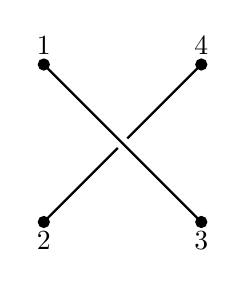
\begin{tikzpicture}
            \draw[black,thick] (-1,-1) -- (-.06,-.06);
            \draw[black,thick] (.06,.06) -- (1,1);
            \draw[black,thick] (-1,1) -- (1,-1);
            \filldraw[black] (-1,-1) circle (2pt) node[anchor=north] {2};
            \filldraw[black] (-1,1) circle (2pt) node[anchor=south] {1};
            \filldraw[black] (1,-1) circle (2pt) node[anchor=north] {3};
            \filldraw[black] (1,1) circle (2pt) node[anchor=south] {4};
        \end{tikzpicture}
    \end{center}
    \captionof{figure}{Marginfigure: Tikz}
    \end{marginfigure}%
    \item \texttt{Margintable:} This environment requires the \texttt{$\backslash$begin\{margintable\}} {$\cdots$}\newline\texttt{$\backslash$end\{margintable\}} enclosings. A table package, such as \texttt{tabular}, \texttt{tabulary}, \texttt{tabu}, or \texttt{tabularx} is required. The \texttt{caption} package is needed to caption the table.
    \begin{margintable}
        \vspace{.1in}
        \begin{tabularx}{\marginparwidth}{|X|X|}
        \hline
        \textit{NotesTeX} & \textbf{rocks!}\\
        \hline
        \end{tabularx}
        \caption{Margintable}
    \end{margintable}
\end{enumerate}
